\clearpage
\section{Final Dataset}
Upon analysing the available datasets, it was 
decided to use several of them for specific purposes. 
The first and most important is the dataset by \textit{Pan et al.}
\ref{section:Pan et al}, 
which is among the most cited and widely reused in various 
benchmarks within this domain. As such, it was used in 
conjunction with the \textbf{testing framework} described in 
Section~\ref{section:Test framework} to obtain a dataset 
suitable for evaluating potential differences between 
functional and non-functional code.

\textit{CodeMirage} \ref{section:CodeMirage} is a 
high-quality dataset and has 
been taken as a reference for future analyses. Despite 
containing the largest number of samples, 
\textit{CoDet-M4} \ref{section:CoDet-M4} 
was excluded from testing due to the unreliability of its 
results. Analysing the entire dataset to identify potential 
issues would be unfeasible; however, it may still represent 
a valuable resource for training machine learning-based 
detection methods.

Finally, \textit{AiGCodeSet} \ref{section:AiGCodeSet} 
remains a potentially useful 
dataset for testing purposes, although it does not contribute 
any additional information beyond what is already provided 
by Pan et al.\ and CodeMirage.

%%%
\subsection{Pan et al tested}
The analysis of the dataset by Pan et al.\ 
enabled the construction of a small dataset 
consisting of definitively correct and definitively 
incorrect code samples (where “incorrect” refers to 
cases in which the LLM-generated code did not produce 
the same outputs as the corresponding human-written code).

The process began with the subset of the dataset 
corresponding to the prompt \textit{“Removal of 
stop words from the prompt”}, which includes 5069 
samples. From this subset, we discarded all code 
samples that the framework was unable to process. 
Tests were then executed on the remaining samples, 
and only those which did not produce runtime faults 
were retained—this was necessary to exclude failures 
due to incorrectly generated tests or missing import 
statements.

As a result, a dataset of approximately 1000 code 
samples was obtained, of which around 600 were 
classified as correct and 400 as incorrect (i.e., 
they failed at least one test).



\begin{figure}[H]
    \centering
    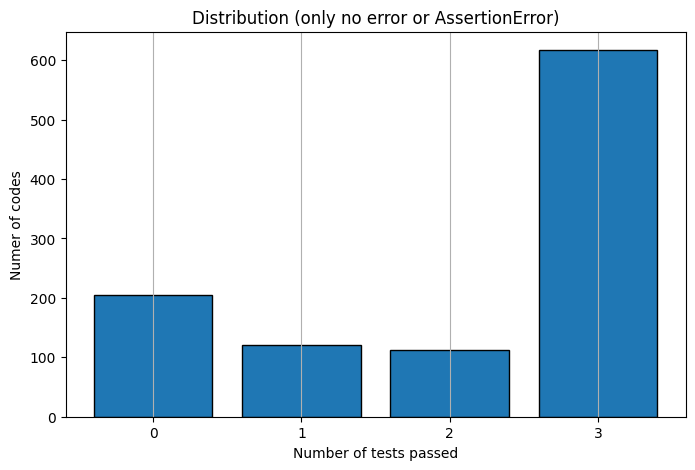
\includegraphics[width=0.6\textwidth]{img/panetaltest/600600.png}
    \caption{Source distribution}
    \label{fig:panetaltest_600600}
\end{figure}